\documentclass{article}
\usepackage{graphicx}
\usepackage[top=10mm, bottom=25mm, left=30mm, right=30mm, includehead]{geometry}
\usepackage{fancyhdr}
\usepackage{mathptmx}
\usepackage{xcolor}
\let\negmedspace\undefined
\let\negthickspace\undefined
\usepackage{../gvv-book}
\usepackage{../gvv}
\usepackage{bm}
\usepackage{cite}
\usepackage{amsmath,amssymb,amsfonts,amsthm}
\usepackage{algorithmic}
\usepackage{textcomp}
\usepackage{listings}
\usepackage{enumitem}
\usepackage{mathtools}
\usepackage{gensymb}
\usepackage{comment}
\usepackage[breaklinks=true]{hyperref}
\usepackage{tkz-euclide}                                    
\usepackage[utf8]{inputenc}                           
\usepackage{color}                                            
\usepackage{array}                                            
\usepackage{longtable}       
\usepackage{calc}                                             
\usepackage{multirow}                       
\usepackage{hhline}                                           
\usepackage{ifthen}                                       
\usepackage{lscape}
\usepackage{tabularx}
\usepackage{float}
\usepackage{multicol}
\usepackage[T1]{fontenc}
\pagestyle{fancy}
\fancyhf{}
\date{}
\setlength{\headheight}{23.10004pt}

\fancypagestyle{plain}{
    \fancyhead[R]{\textit{$4^{th}$ International Conference on Recent Advances in Applied Mathematics (RAAM2026)\\ 6--8 July $2026$, Indian Institute of Technology, Hyderabad}}
    \renewcommand{\headrulewidth}{0pt}
    }
\onecolumn
\bibliographystyle{IEEEtran}
\numberwithin{equation}{section}
\numberwithin{figure}{section}
\renewcommand{\thetable}{\theenumi}

\title{\bfseries\large{A Logo for Narayanpal}}

\author{\underline{Subhodeep Chakraborty}\footnote{Department of Electrical Engineering, Indian Institute of Technology, Hyderabad}, Shiven Bajpai\footnote{Department of Artifical Intelligence, Indian Institute of Technology, Hyderabad} and G.V.V. Sharma\footnote{Department of Electrical Engineering, Indian Institute of Technology, Hyderabad}}

\begin{document}
\maketitle
%\vspace{-0.7cm}

\begin{abstract}
This paper outlines a rigorous mathematical framework for generating a unique visual logo. Unlike conventional graphic design techniques that rely on free-form vector drawing, this approach derives a foundational geometric structure by linking a continuous-time signal's integral constraints to the analytic geometry of conic sections using matrix equations and decompositions. Specifically, we extract the decay parameters of an exponential signal by mapping them to the latus recta endpoints of a derived hyperbola. A precise truncation method based on decibel attenuation is then applied to the resulting infinite waveform to yield a bounded, aesthetic visual asset usable as a logo.
\end{abstract}

%\vspace{0.1cm}
\section*{1. Introduction and Related Work}
Many companies map explicit equations to their brand, such as Broadcom's stylized sinc function ($\operatorname{sinc}(x)$) and Cisco's discrete digital waveforms.%\footnote{A. Smith and J. Doe, \emph{J. of Visual Branding} \textbf{45}, 112 (2018).} 
In algorithmic graphics, mathematical frameworks generally take two forms. The first is generative: utilizing parametric primitives, double pendulum kinematics, or trigonometry to script interactive patterns for textiles and digital art.\footnote{P. Jha and B. B. Biswal, \emph{J. of Graphic Eng. and Design} \textbf{11}, 37 (2020).}\footnote{I. Staribratov and N. Manolova, \emph{Math. and Informatics} \textbf{65}, 72 (2022).} The second is proportional: applying recursive sequences like the Golden Ratio, or simplified 2:3:5 geometric ratios, to refine manually drawn Bézier curves.\footnote{M. Rizaldi and R. Anthonius, \emph{Adv. in Soc. Sci., Edu. and Hum. Res.} \textbf{502}, 21 (2020).} 

Despite these methodologies, a significant gap persists: existing mathematical logo designs either serve as proportional overlays to hand-drawn vector art or employ generative scripts that ultimately require arbitrary aesthetic cropping within design software. This project overcomes this by introducing a purely mathematical approach from start to finish. Rather than relying on drawing tools or visual grids, the logo's exact structural coordinates were analytically derived directly from signal processing constraints and eigenvalue decomposition. Furthermore, arbitrary software masking was replaced with precise signal truncation derived from  attenuation limits. This ensures the final visual asset is not merely mathematically assisted, but strictly mathematically generated.

% often translate mathematical functions directly into visual identities; for instance, Broadcom employs a stylized sinc function ($\operatorname{sinc}(x)$) to represent an ideal low-pass filter,\footnote{A. Smith and J. Doe, \emph{J. of Visual Branding} \textbf{45}, 112 (2018).} while Cisco merges a discrete digital waveform with the suspension geometry of the Golden Gate Bridge.\footnote{M. Weaver, \emph{Digital Waveforms in Art}, Tech Press (2020).} Foundational designs for consumer brands like Apple famously utilize the Fibonacci sequence and the Golden Ratio to achieve aesthetic perfection.\footnote{R. Evans et al., \emph{J. of Design Proportions} \textbf{22}, 15 (2015).} In academia, the National Institute of Advanced Studies (NIAS) bases its emblem on the \textit{śyenaciti}, an ancient geometric Vedic fire altar,\footnote{R. Narasimha, \emph{NIAS News} \textbf{8}, 2 (1999).} and computer science projects like MathSeer integrate equations directly into their user interface architectures.\footnote{R. Dmello, \emph{J. of Math UI} \textbf{4}, 102 (2019).} 

%Building upon this legacy of using proportional overlays or explicit functional graphs, our paper proposes a novel synthesis. Instead of relying on parametric primitives or isolated formulas, we derive a logo's exact structural coordinates by leveraging continuous-time signal processing constraints alongside eigenvalue decomposition. Our method mandates that the visual shape is the strict analytical outcome of a converging area integral.

%\vspace{0.1cm}
\section*{2. Mathematical Formulation}
The logo's underlying structure is defined by the continuous-time function $f(t) = e^{-at}u(t) + e^{bt}u(-t)$. The parameters $(a,b)$ are derived by enforcing a constraint for unit area, yielding the conic section $ab - a - b = 0$. By expressing this conic in the standard quadratic form $\text{g}(\vec{x}) = \vec{x}^\text{T}\vec{Vx} + 2\vec{u}^\text{T}\vec{x} + f$ and performing eigendecomposition, we apply affine transformations to map the hyperbola into a standard coordinate system. The parameters $(a,b)$ are then explicitly chosen as the valid endpoints of the latus recta of this conic, yielding a precise solution.% $\vec{\hat{x}}_1 = \myvec{2+\sqrt{2} \\ \sqrt{2}}$. 

%\vspace{0.1cm}
\section*{3. Logo Realization and Truncation}
Because the derived function $f(t)$ extends to infinity, it must be strategically truncated to serve as a practical logo. Rather than arbitrary cropping, a $-30$dB amplitude attenuation threshold was enforced to derive theoretical truncation bounds $t_1$ and $t_2$ precisely. The resulting bounded graph was taken as the final mathematically synthesised logo.

\iffalse
\vfill
\begin{figure}[H]
	\centering
	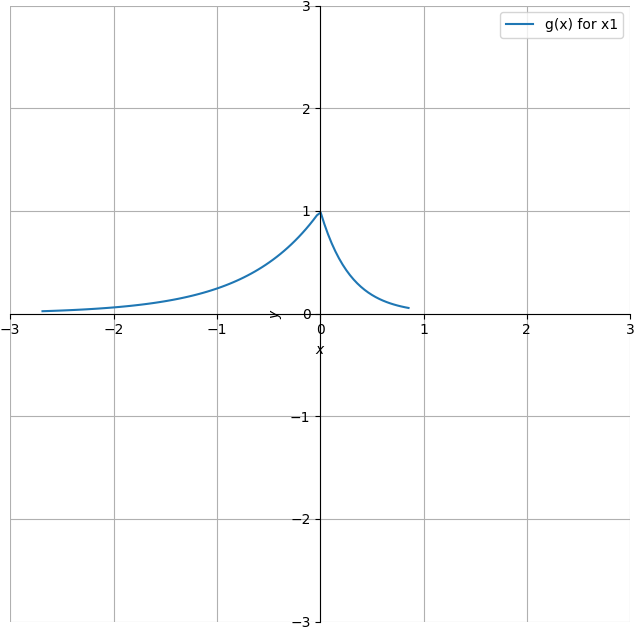
\includegraphics[width=0.55\columnwidth]{../figs/trunc.png}
	\caption{The final truncated logo generated from the derived parameters $(a,b)$.}
	\label{fig:Truncation}
\end{figure}
\fi
\end{document}
